\documentclass[11pt]{article}

\usepackage{amsmath,amssymb,amsthm}
\usepackage{xcolor}
\usepackage{tikzit}
\usepackage[backend=biber]{biblatex}
\addbibresource{references.bib}
\usepackage{hyperref}

% Colours used in zx.tikzstyles
\definecolor{zxred}{RGB}{232, 165, 165}
\definecolor{zxgreen}{RGB}{216, 248, 216}
\definecolor{zxhad}{RGB}{255, 255, 130}
\definecolor{zxpaulibox}{RGB}{221, 221, 255}
\input{zx.tikzstyles}

\newcommand{\scalareq}{\ensuremath{\propto}}  % used in figures/bialgebra-rule.tikz

% A macro drawing a TikZ picture, with an optional argument: a spider of the given colour with a phase.
% tikz2html --init finds it, and its arguments.
\newcommand{\spider}[2][Z]{\tikz[baseline=-0.6ex]{\node[style=#1 phase dot] {$#2$};}}

\newtheorem{proposition}{Proposition}

\title{Phase gadgets: a short example paper}
\author{tikz2html}

\begin{document}
\maketitle

\begin{abstract}
  An example of a paper converted to html with tikz2html: it has figures made with TikZiT and with plain TikZ,
  in equations, in the text and in figures, and sections in separate files.
\end{abstract}

\section{Introduction}\label{sec:intro}

ZX-diagrams~\cite{CoeckeDuncan2011} are built from spiders, like $\spider{\alpha}$ and $\spider[X]{\beta}$.
Two spiders of the same colour fuse, adding their phases:
\begin{equation}\label{eq:fusion}
  \tikzfig{spider-fusion-Z}
\end{equation}
Spiders of different colours satisfy the bialgebra rule:
\begin{equation}\label{eq:bialgebra}
  \tikzfig{bialgebra-rule}
\end{equation}

Plain TikZ works too, also outside of the figures made with TikZiT, as in Figure~\ref{fig:circuit}.
\begin{figure}[ht]
  \centering
  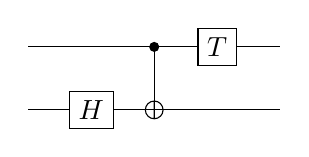
\begin{tikzpicture}[scale=0.8]
    \draw (0,0) -- (4,0) (0,1) -- (4,1);
    \draw (2,0) -- (2,1);
    \filldraw (2,1) circle (2pt);
    \draw (2,0) circle (4pt) (2,-0.14) -- (2,0.14);
    \node[draw, fill=white] at (1,0) {$H$};
    \node[draw, fill=white] at (3,1) {$T$};
  \end{tikzpicture}
  \caption{A circuit drawn with plain TikZ. Inline: \tikz[baseline=-0.6ex]{\draw (0,0) circle (3pt);}.}
  \label{fig:circuit}
\end{figure}

\section{Phase gadgets}\label{sec:gadgets}

Phase gadgets on the same set of qubits can be fused, which follows from \eqref{eq:fusion} and
\eqref{eq:bialgebra}:
\begin{proposition}\label{prop:gadgets}
  \begin{equation}\label{eq:gadget-fusion}
    \tikzfig{gadget-fusion}
  \end{equation}
\end{proposition}
Using this, a circuit with several gadgets can be simplified step by step, where the references above the
equalities are links:
\begin{align*}
  \tikzfig{phase-gadget-reduced}
  &\overset{\eqref{eq:gadget-fusion}}{=} \tikzfig{phase-gadget-reduced} \\
  &\overset{\text{Prop.~\ref{prop:gadgets}}}{=} \tikzfig{had-had-cancel}
\end{align*}
Section~\ref{sec:intro} has more about the spiders $\spider{\gamma}$.


\printbibliography
\end{document}
